\input{../../../preamble.tex}
% \bibliographystyle{plain} % Style BST file (bmc-mathphys, vancouver, spbasic).
% \bibliographystyle{unsrt} % Style BST file (bmc-mathphys, vancouver, spbasic).
% \bibliography{pubs.bib}      % Bibliography 
\bibliography{pubs.bib}
\title{Motorstyring bidrag}
\author{Simon Mylius Rasmussen}

\begin{document}

\lstset{language=C,%
  % basicstyle=\color{red},
  breaklines=true,%
  morekeywords={matlab2tikz},
  keywordstyle=\color{blue},%
  morekeywords=[2]{1}, keywordstyle=[2]{\color{black}},
  identifierstyle=\color{black},%
  stringstyle=\color{mylilas},
  commentstyle=\color{mygreen},%
  showstringspaces=false,%without this there will be a symbol in the places where there is a space
  % numbers=left,%
  % numberstyle={\tiny \color{black}},% size of the numbers
  % numbersep=9pt, % this defines how far the numbers are from the text
  emph=[1]{for,end,break},emphstyle=[1]\color{red}, %some words to emphasise
  % emph=[2]{word1,word2}, emphstyle=[2]{style},    
}
% \lstdefinestyle{customc}{
%   belowcaptionskip=1\baselineskip,
%   breaklines=true,
%   frame=L,
%   xleftmargin=\parindent,
%   language=C,
%   showstringspaces=false,
%   basicstyle=\footnotesize\ttfamily,
%   keywordstyle=\bfseries\color{green!40!black},
%   commentstyle=\itshape\color{purple!40!black},
%   identifierstyle=\color{blue},
%   stringstyle=\color{orange},
% }

% \lstdefinestyle{customasm}{
%   belowcaptionskip=1\baselineskip,
%   frame=L,
%   xleftmargin=\parindent,
%   language=[x86masm]Assembler,
%   basicstyle=\footnotesize\ttfamily,
%   commentstyle=\itshape\color{purple!40!black},
% }

% \lstset{escapechar=@,style=customc}

\newcounter{udrboks}[section]\setcounter{udrboks}{0}
\renewcommand{\theudrboks}{\arabic{section}.\arabic{udrboks}}
\renewcommand{\theudrboks}{\arabic{udrboks}}
\newenvironment{udrboks}[2][]{%
  \refstepcounter{udrboks}%
  \ifstrempty{#1}%
  {\mdfsetup{%
      frametitle={%
        \tikz[baseline=(current bounding box.east),outer sep=0pt]
        \node[anchor=east,rectangle,fill=blue!20]
        {\strut Udregninger~\theudrboks};}}
  }%
  {\mdfsetup{%
      frametitle={%
        \tikz[baseline=(current bounding box.east),outer sep=0pt]
        \node[anchor=east,rectangle,fill=blue!20]
        {\strut Udregninger ~\theudrboks:~#1};}}%
  }%
  \mdfsetup{innertopmargin=10pt,linecolor=blue!20,%
    linewidth=2pt,topline=true,%
    frametitleaboveskip=\dimexpr-\ht\strutbox\relax
  }
  \begin{mdframed}[]\relax%
    \label{#2}}{\end{mdframed}}


\newcounter{formelboks}[section]\setcounter{formelboks}{0}
\renewcommand{\theformelboks}{\arabic{section}.\arabic{formelboks}}
\renewcommand{\theformelboks}{\arabic{formelboks}}
\newenvironment{formelboks}[2][]{%
  \refstepcounter{formelboks}%
  \ifstrempty{#1}%
  {\mdfsetup{%
      frametitle={%
        \tikz[baseline=(current bounding box.east),outer sep=0pt]
        \node[anchor=east,rectangle,fill=blue!20]
        {\strut Formler~\theformelboks};}}
  }%
  {\mdfsetup{%
      frametitle={%
        \tikz[baseline=(current bounding box.east),outer sep=0pt]
        \node[anchor=east,rectangle,fill=blue!20]
        {\strut Formler ~\theformelboks:~#1};}}%
  }%
  \mdfsetup{innertopmargin=10pt,linecolor=blue!20,%
    linewidth=2pt,topline=true,%
    frametitleaboveskip=\dimexpr-\ht\strutbox\relax
  }
  \begin{mdframed}[]\relax%
    \label{#2}}{\end{mdframed}}

\newcounter{konstboks}[section]\setcounter{konstboks}{0}
\renewcommand{\thekonstboks}{\arabic{section}.\arabic{konstboks}}
\newenvironment{konstboks}[2][]{%
  \refstepcounter{konstboks}%
  \ifstrempty{#1}%
  {\mdfsetup{%
      frametitle={%
        \tikz[baseline=(current bounding box.east),outer sep=0pt]
        \node[anchor=east,rectangle,fill=green!20]
        {\strut Konstanter~\thekonstboks};}}
  }%
  {\mdfsetup{%
      frametitle={%
        \tikz[baseline=(current bounding box.east),outer sep=0pt]
        \node[anchor=east,rectangle,fill=green!20]
        {\strut Konstanter~\thekonstboks:~#1};}}%
  }%
  \mdfsetup{innertopmargin=10pt,linecolor=green!20,%
    linewidth=2pt,topline=true,%
    frametitleaboveskip=\dimexpr-\ht\strutbox\relax
  }
  \begin{mdframed}[]\relax%
    \label{#2}}{\end{mdframed}}
\pgfplotstableread[row sep=\\,col sep=&]{
  ide & stemmer  \\
  Paraply & 9  \\
  Fjernbetjening & 7  \\
  iAdapt & 2 \\
}\mydata
% \setcounter{secnumdepth}{1}
\maketitle
\thispagestyle{empty}

% \textbf{Deltagere:}
% \begin{figure}[h]
%   \centering
%   % BEGIN RECEIVE ORGTBL delt
%   \begin{tabular}{|p{5cm}p{10cm}|}
%     \hline
%     &\\
%     Stud. nr: 201602094 & Navn: Søren Holm Korsgaard \\
%     \hline
%     &\\
%     Stud.nr.: 201607563 & Navn: Jacob Gustafsson \\
%     \hline
%     &\\
%     Stud.nr.: 201704859 & Navn: Jonas Buus \\
%     \hline
%     &\\
%     Stud.nr.: 20084327 & Navn: Simon Rasmussen \\
%     \hline
%     &\\
%     Stud.nr.: 201704483 & Navn: Thomas Dueholm Jensen \\
%     \hline
%   \end{tabular}
%   % END RECEIVE ORGTBL delt

% \end{figure}
\vspace{-5mm}
% \clearpage
\setcounter{tocdepth}{2}
\tableofcontents
\thispagestyle{empty}
\newpage
% \pagenumbering{arabic}
\setcounter{page}{1}

% \section{Introduktion}
% \label{sec:introduktion}

\section{Baggrund}
\label{sec:baggrund}

Motorstyringen for systemet vil bestå i præcis justering af forbrændingsmotorens omdrejninger i forhold til dronecopterens strømforbrug. Det valgtes at arbejde med et simplere system for at fokuserer på principperne i motorstyring. Det betød at motorstyringen skulle bestå i udvikling af PID-regulering af forbrændingsmotoren sådan at der skulle foregå korrektion af motorens spjældvinkel i forhold til motorens omdrejninger.

Fjare\autocite{pid1} er en artikel der beskriver PID regulering af en forbrændingsmotor som skal drive en aerocopter. Der er taget inspiration fra denne tilgang inklusiv PID-regulering og PID-koefficienter.
% Målet med dette afsnit er at opstille en kravsspecifikation for motorstyringen samt at færdiggøre analysen af motorstyringen og lægge op til hvordan en test af motorstyring kan udformes for at præcisere PID-algoritme samt at opfylde krav.

% \lstdefinestyle{customc}{
%   belowcaptionskip=1\baselineskip,
%   breaklines=true,
%   frame=L,
%   xleftmargin=\parindent,
%   language=C,
%   showstringspaces=false,
%   basicstyle=\footnotesize\ttfamily,
%   keywordstyle=\bfseries\color{green!40!black},
%   commentstyle=\itshape\color{purple!40!black},
%   identifierstyle=\color{blue},
%   stringstyle=\color{orange},
% }

% \lstdefinestyle{customasm}{
%   belowcaptionskip=1\baselineskip,
%   frame=L,
%   xleftmargin=\parindent,
%   language=[x86masm]Assembler,
%   basicstyle=\footnotesize\ttfamily,
%   commentstyle=\itshape\color{purple!40!black},
% }

% \lstset{escapechar=@,style=customc}

\subsection{Kravsspecifikation}
\label{sec:kravsspecifikation}
Med baggrund i Fjare\autocite{pid1} sættes følgende krav:
\begin{itemize}
\item Overshoot skal ikke være mere en 197 rpm.
\item Justeringstiden må max være 8,8 sekunder.
\item Ifm. et step respons skal 90 \% af målet være opnået i mindre end 3 sekunder.
\item Det skal være muligt at vedligeholde en konstant hastighed over længere tid (dvs. mere end 5 minutter).
\item Servomotoren skal kunne reguleres.
\item Motoren skal kunne startes.
\item Omdrejningerne skal kunne måles.
\end{itemize}

\subsection{PID regulering}
\label{sec:overordnet-mal}

PID-regulering består i regulering af et output på baggrund af forskellen mellem det tilstræbte og det faktiske - dette kan kaldes fejlen. PID regulering kan beskrives med
\begin{equation}
  \label{eq:1}
  u(t)=k_Pe(t)+k_I \int_0^t e(\tau)\mathrm{d}\tau + k_D\frac{\mathrm{d}e(t)}{\mathrm{d}t}
\end{equation}

hvor $e(t)$ er fejl som funktion af tiden, $e(\tau)$ er fejl som funktion af den akkumulerede tid og $k_P$, $k_I$ og $k_D$ er koefficienter svarende til henholdsvis det proportionale, integrede og deriverede forhold. Det proportionale vil sige forholdet mellem tilstræbte og det faktiske for et givent tidspunkt. Det integrede vil sige forskellen mellem tilstræbte og det faktiske akkummuleret over tid. Det betyder at den integrerede koefficient viser en trend for fejlen. Det deriverede er et mål for hvor hurtigt fejlen ændrer sig over tid.

Formålet ved udarbejdelse af PID-regulering er at finde de optimale værdier af $k_P$, $k_i$ og $k_d$.

% For et givent sæt af K-værdier, udvælges en række forskellige typer af trinvise ændringer i hastigheden. Der måles på hvor lang tid det tager for ændringen at indfinde sig, samt hvor store udsving dette gør sig ud i.

Som udgangspunkt er det tidligere vist(\autocite{pid1}) at $K_p=0,065$ og $K_i=0,000005$ har været optimale, samt at $K_d$ helt blev droppet eftersom det ikke var en gavnlig parameter.

\subsection{Software}
\label{sec:software}

Fra Fjare\autocite{pid1} kunne et eksempel på et program være skrevet i pseudo C-kode:
\begin{lstlisting}[language=C,basicstyle=\ttfamily]
  void velPID ( ) {
    lowpassSpeed = alpha * lastLowpassSpeed + (1-alpha) * measuredSpeed;
    K1 = kp * setpointWeight * (setpointSpeed - lastSetpointSpeed) + kp * (lastMeasuredSpeed - lowpassSpeed);
    K2 = ki * (setpointSpeed - lowpassSpeed);
    K3 = kd * (2 * lastMeasuredSpeed - lowpassSpeed - lastLastMeasuredSpeed);
    output = lastOutput - K1 - K2 - K3;
    throttlePos = floor(output + 0.5);
    if(throttlePos<throttleopen){
      output = (double) throttleopen;
      throttlePos=throttleopen;
    }
    if(throttlePos>throttlesafe){
      output = ( double )throttlesafe;
      throttlePos=throttlesafe;
    }
    lastLowpassSpeed = lowpassSpeed;
    lastLastMeasuredSpeed = lastMeasuredSpeed;
    lastMeasuredSpeed = lowpassSpeed;
    lastSetpointSpeed = setpointSpeed;
    lastOutput = output;
    throttle.writeMicroseconds(throttlePos);
  }
\end{lstlisting}


\section{Metode og analyser}
\label{sec:metode}

\subsection{Stepinput og overføringsfunktion}
\label{sec:tests}

PID-koefficienterne skal defineres udfra en overføringsfunktion for vores system som skal reguleres. For at udlede overføringsfunktionen blev et forsøg med optagelse af steprespons udarbejdet.

% Et testprogram kan køres via microcontroller som foretager PID-reguleringen og optage motorens omdrejninger ved forskellige skift mellem hastigheder. Disse gentages for forskellige værdier af $K_p$ og $K_i$.

Som udgangspunkt skulle det interessante for dronecopteren være at % I en teststand vil formålet være at test forskellige værdier af koefficienterne og i forskellige kombinationer. Målet med PID-reguleringen er at
strømmen fra batteri til dronens propelmotorer er konstant. Tilgengæld skal spjældet til forbrændingsmotoren konstant reguleres. Derfor vil en teststand som udgangspunkt have følgende:
\begin{itemize}
\item input: strøm fra batteri til drone
\item output: regulering af spjæld via servomotor
\end{itemize}

Her vil $e(t)$ være et mål for forskellen mellem den ønskede strømstyrke og den faktiske.

Det var ikke muligt at måle strømmen fra batteri til drone. For at lave en teststand som kan tjene som demonstration af PID-regulering samt som skabelon for senere tests fremstilles istedet en teststand som skal justere spjældet i forhold til motorens omdrejninger. Dvs:

\begin{itemize}
\item input: motorens omdrejninger
\item output: regulering af spjæld via servomotor
\end{itemize}

I dette tilfælde vil $e(t)$ være et mål for forskellen mellem det ønskede omdrejningstal og det faktiske.

For at få en grov ide om niveauet af koefficienterne kan en simulink simulation være gunstig. I denne skal gøres en række antagelser af forholdet mellem spjældvinkel og omdrejningstallet. Når koefficienterne er tunet i simulink kan der laves en test.

% I testen skal der laves forskellige trinsvise ændringer af omdrejningstallet. Fjare\autocite{pid1} har beskrevet hvordan 4 forskellige trinmønstre (se figur\ref{fig:paths}) blev brugt til at justere en PID-algoritme som blev brugt til en forbrændingsenhed i en ubemandet flyvende enhed.

% \begin{figure}[h]
%   \centering
%   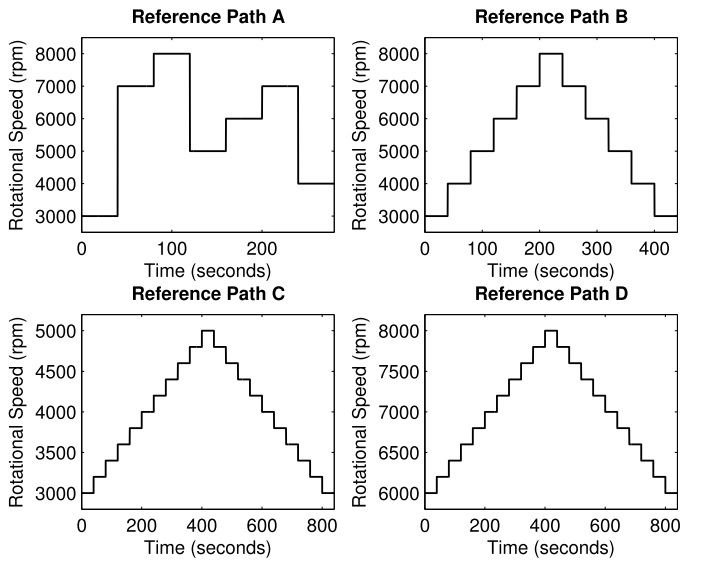
\includegraphics[width=0.7\textwidth]{refpaths.JPG}
%   \caption{Trinmønstre}
%   \label{fig:paths}
% \end{figure}

% På trods af at forbrændingsenheden altså ikke opladet batteri virker det relevant at tage udgangspunkt i lignende trinmønste til PID-kontrol af motoromdrejninger.

% KL25 vil tjene både som microcontroller og datalogger.

\subsubsection{Steprespons}
\label{sec:steprespons}

%For at simplificere PID-reguleringen forsøges forst med regulering af spjæld i forhold til motorens omdrejninger.
Der vil tages udgangspunkt i måling af et steprespons på motorens omdrejninger. Til målinger af omdrejninger anvendtes et oscilloskop som optog data fra Hall-sensoren. Optagelsen blev tricket fra KL25Z.% foreslås at bruge Pocketbeagle som vil kunne foretage måling af omdrejninger via Hall-sensor og lagre data i en fil som kan eksporteres til analyse i Matlab.

Data fra oscilloskopet bestod i 50000 målinger som bestod af Hall-sensorens spænding, spændingen fra servomotoren, der styrer spjældet, samt et tidsmål. Nedenfor ses et udsnit af de 50000 målinger:

\begin{table}[h]
  \centering
% BEGIN RECEIVE ORGTBL tabel4
\begin{tabular}{r|r|r}
\hline
\textbf{second} & \textbf{Volt} & \textbf{Volt1} \\
\hline
-1 & 0.215206000000000 & 4.98492460000000 \\
-0.999900000000000 & 0.215206000000000 & 4.90452260000000 \\
-0.999800000000000 & 0.134804000000000 & 4.90452260000000 \\
-0.999700000000000 & 0.215206000000000 & 4.98492460000000 \\
-0.999600000000000 & 0.215206000000000 & 4.90452260000000 \\
-0.999500000000000 & 0.215206000000000 & 4.90452260000000 \\
-0.999400000000000 & 0.215206000000000 & 4.90452260000000 \\
-0.999300000000000 & 0.215206000000000 & 4.82412060000000 \\
-0.999200000000000 & 0.215206000000000 & 4.90452260000000 \\
\hline
\end{tabular}
% END RECEIVE ORGTBL tabel4
  \caption{}
  \label{tab:komp3}
\end{table}
\begin{comment}
#+ORGTBL: SEND tabel4 orgtbl-to-latex :splice nil :skip 0
|--------------------+-------------------+------------------|
|             second |              Volt |            Volt1 |
|--------------------+-------------------+------------------|
|                 -1 | 0.215206000000000 | 4.98492460000000 |
| -0.999900000000000 | 0.215206000000000 | 4.90452260000000 |
| -0.999800000000000 | 0.134804000000000 | 4.90452260000000 |
| -0.999700000000000 | 0.215206000000000 | 4.98492460000000 |
| -0.999600000000000 | 0.215206000000000 | 4.90452260000000 |
| -0.999500000000000 | 0.215206000000000 | 4.90452260000000 |
| -0.999400000000000 | 0.215206000000000 | 4.90452260000000 |
| -0.999300000000000 | 0.215206000000000 | 4.82412060000000 |
| -0.999200000000000 | 0.215206000000000 | 4.90452260000000 |
|--------------------+-------------------+------------------|
\end{comment}

Spændingen fra Hall-sensoren, Volt1, anvendes.
Når data plottes for et kort tidsrum ses støj omkring 5 volt

\begin{figure}[h]
  \centering
  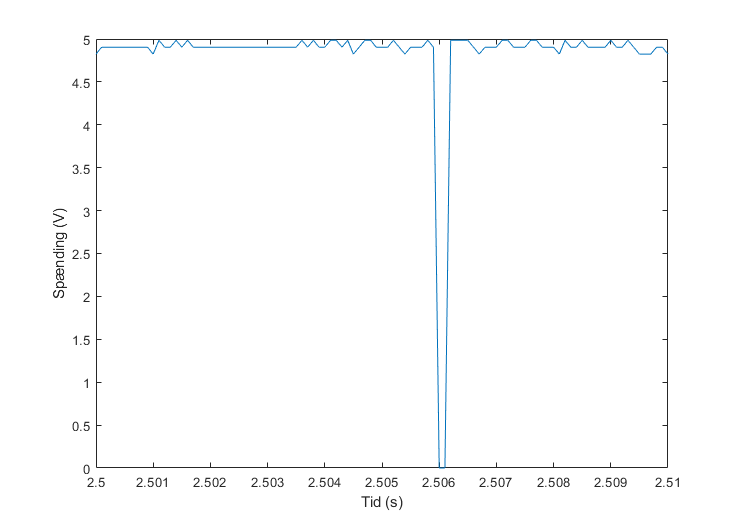
\includegraphics[width=0.6\textwidth]{mo1.png}
  \caption{}
  \label{fig:mo1}
\end{figure}

Data processeres nu med følgende Matlab-script:
\begin{lstlisting}[language=Matlab]
close all
data = stepdata5;
t = data.second;
v = data.Volt1;
border1 = 4.5;
border2 = 0.1;
v2 = data.Volt;
b = 0;
stop = 0;
tp = [];
tpt = [];
vpt0 = [];
i = 1;
nyv = [];
while (i <= length(t))
    if (v(i)>border1)
        vn = 5;
    else
        vn = 0;
    end
    nyv = [nyv vn];
    i = i + 1;
end
i = 1;


while (i < length(t))
    if ((nyv(i+1)>border1 & nyv(i)<border2) & b == 0)
        t1 = t(i+1);
        stop = 1;
        b = 1;
    end
    i = i + 1;
    vpt0 = [vpt0 0];
    while (stop ~= 2 & b == 1 & i < length(t))
        if (stop == 1)
            while (stop ~= 2 & i < length(t))
                if (nyv(i+1)>border1 & nyv(i)<border2)
                    t2 = t(i+1);
                    stop = 2;
                end
                i = i + 1;
                vpt0 = [vpt0 0];
            end
        end
        if (stop == 2)
            period = t2-t1;
            tpt = [tpt t2];
            vpt0(i) = nyv(i);
            tp = [tp period];
            t1 = t2;
            stop = 1;
        end
    end
end  
\end{lstlisting}

I scriptet fortolkes spænding over 4,5 V som 5 V. Markering af periodegrænser ved 5 Volt kan ses her (de røde prikker øverst):

\begin{figure}[h]
  \centering
  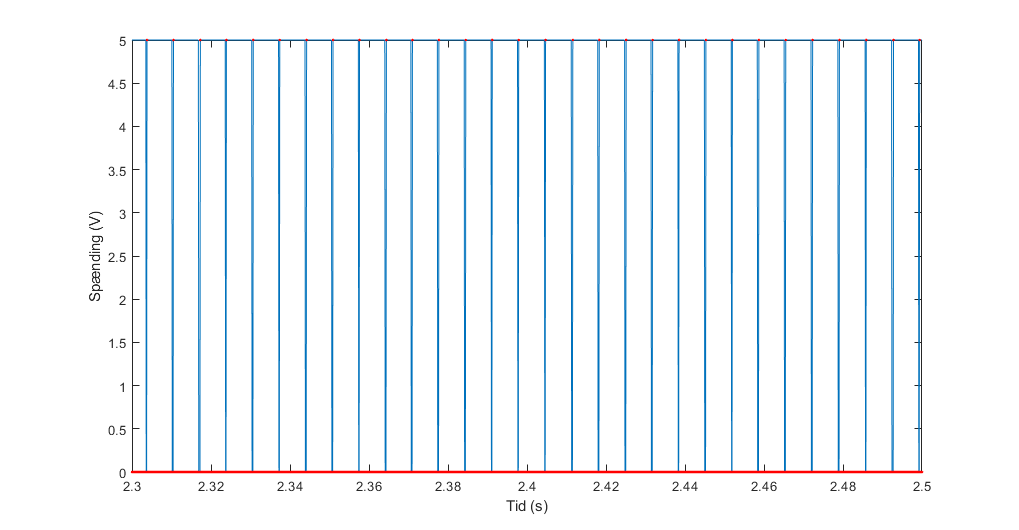
\includegraphics[width=0.6\textwidth]{mo2.png}
  \caption{}
  \label{fig:mo2}
\end{figure}

Herudover udregnes tiden for hver omdrejningsperiode og gemmes i vektoren ”tp”.
Ved plot at tp givet ved rpm overfor tid fås:

\begin{figure}[h]
  \centering
  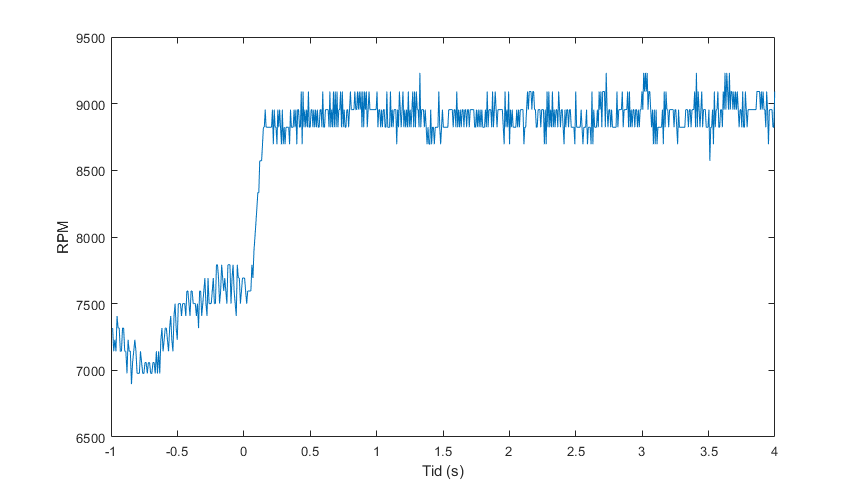
\includegraphics[width=0.6\textwidth]{mo3.png}
  \caption{}
  \label{fig:mo3}
\end{figure}

\subsubsection{Overføringsfunktion}
\label{sec:overforingsfunktion}
Udfra stepresponset skal følgende identificeres:

\begin{itemize}
\item Rise time, $t_r$
\item Settling time, $t_s$
\item Overshoot, $M_p$
\item Peak time, $t_p$
\end{itemize}

Scopet der har målt data gemmer også data op til stepresponset. Stepresponset ses ved tiden 0.
Ved at applicere et midlingsfilter på 200 fås et indtryk af et steady-state niveau ved 8900, med start fra 7600, dvs 1300. 

\begin{figure}[h]
  \centering
  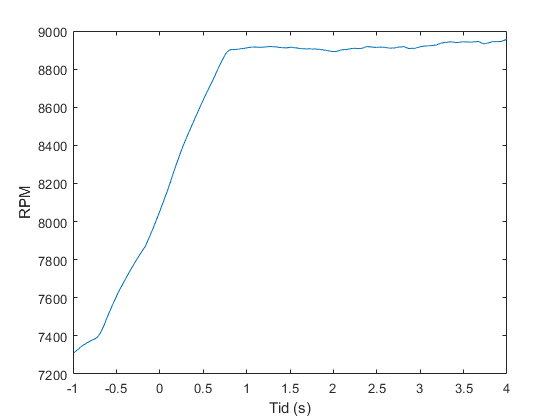
\includegraphics[width=0.5\textwidth]{mo4.png}
  \caption{}
  \label{fig:mo4}
\end{figure}

Ved at applicere et midlingsfilter på 10 fås et indtryk af en 1. grads overføringsfunktion.

\begin{figure}[h]
  \centering
  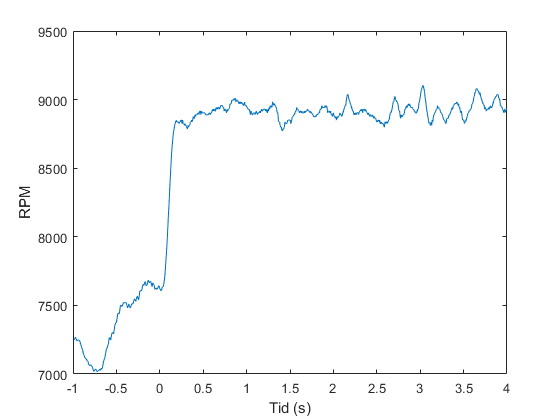
\includegraphics[width=0.5\textwidth]{mo5.png}
  \caption{}
  \label{fig:mo5}
\end{figure}

Det måles at steady-state er opnået ved 0,19 sekunder. Dvs. $0.81 = 5\tau \Leftrightarrow \frac{0,19}{5}=\tau=0,04$.

Hermed kan overføringsfunktionen sættes som
\begin{equation}
  \label{eq:1}
G(s) = \frac{1300}{0,04s+1}  
\end{equation}

% I sidste timebox fandtes overføringsfunktionen
% \begin{equation}
%   \label{eq:1}
% G(s) = \frac{8900}{0,04s+1}  
% \end{equation}
\clearpage
I Simulink oprettes følgende:

\begin{figure}[h]
  \centering
  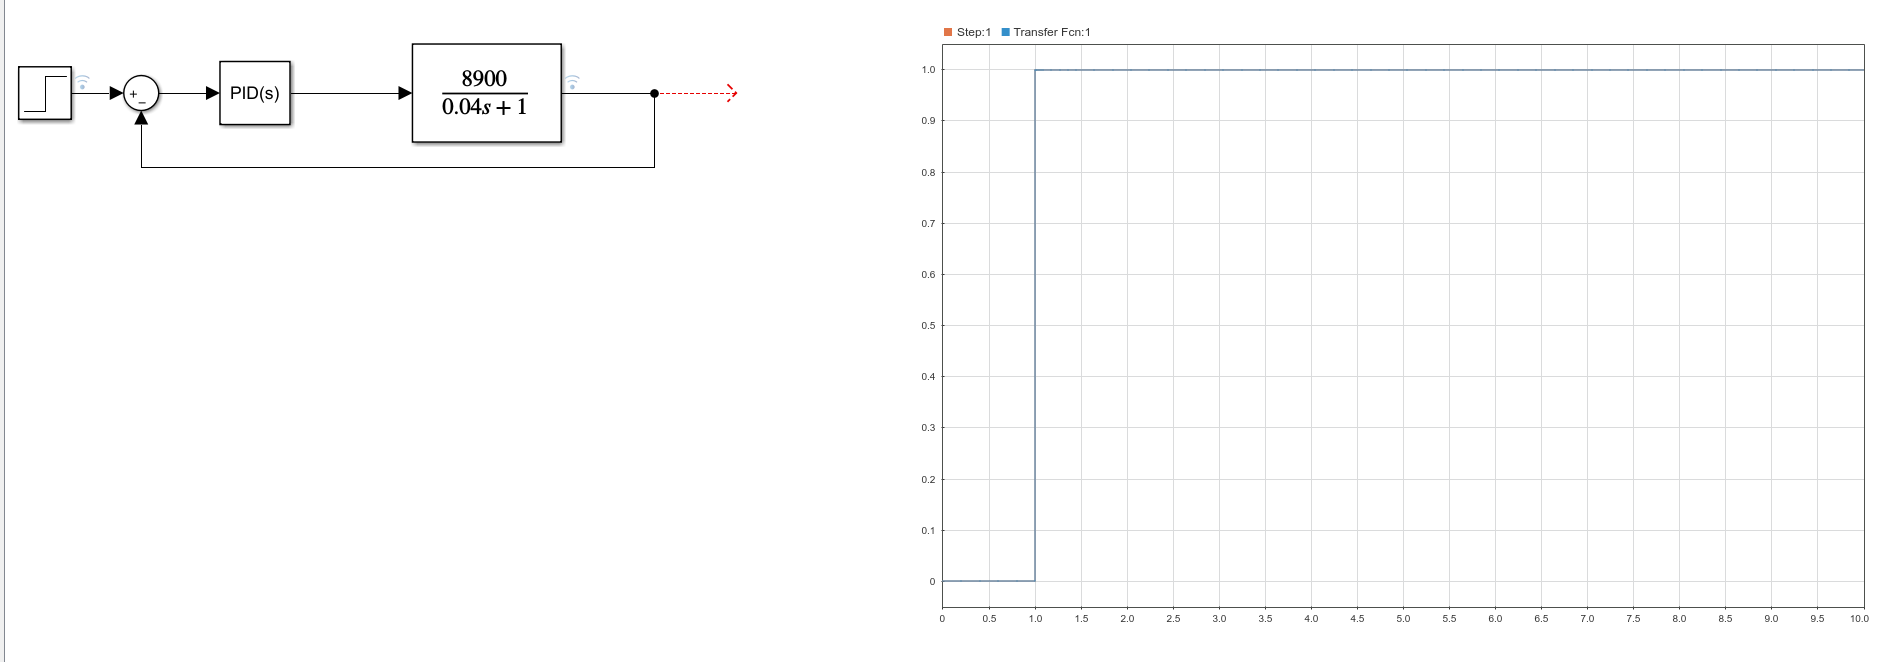
\includegraphics[width=0.6\textwidth]{sbil1.png}
  \caption{Simulink - diagram}
  \label{fig:sbil1}
\end{figure}

Herefter laves autotuning i PID-modulet. Der findes koefficienter svarende til $P=0,0010$, $I=0,0514$, $D=-1,4946$ og følgende respons:

\begin{figure}[h]
  \centering
  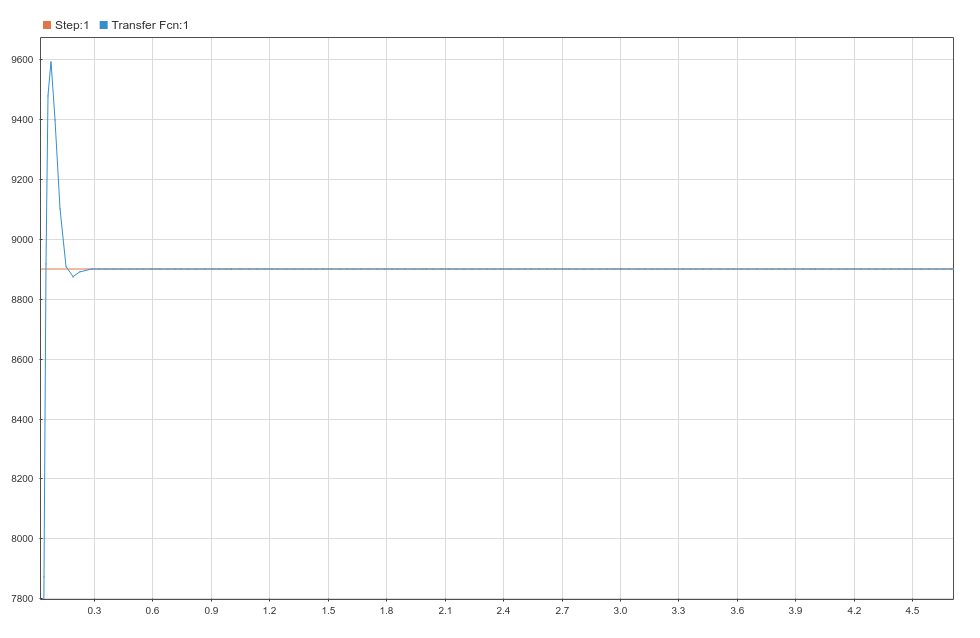
\includegraphics[width=0.6\textwidth]{sbil2.png}
  \caption{Simulink - diagram 2}
  \label{fig:sbil1}
\end{figure}

\subsection{Software}
\label{sec:software-1}

Der udarbejdes nu et udkast til PID-kontrol software som også benytter sig af software til kontrol af servomotor samt aflæsning af motorens omdrejninger (se afsnit XXX).

\begin{lstlisting}[language=C,basicstyle=\ttfamily]
#include <stdio.h>
#include "board.h"
#include "peripherals.h"
#include "pin_mux.h"
#include "clock_config.h"
#include "MKL25Z4.h"
#include "fsl_debug_console.h"
#include "rpm-detect.h"
#include "servo_driver.h"

// Filtrering
double alpha = 0.2;
double measuredSpeed = 0 ;

// Koefficienter
double kp = 0.001;
double ki = 0.0514;
double kd = -1.4946;
double K1;
double K2;
double K3;

// Vægtning af koefficienter
double setpointWeight = 0.2;
double lowpassSpeed;
double setpointSpeed;

// Diverse
double output;
double throttleopen = 1.0;
float throttlePos;

int rpmch;
int MAX_RPM = 9000;

// Initialiering
double lastSetpointSpeed = 0;
double lastMeasuredSpeed = 0;
double lastLowpassSpeed = 0;
double lastOutput = 0;
double lastLastMeasuredSpeed = 0;

void velPID (int setpointSpeed, int measuredSpeed) {
    lowpassSpeed = alpha * lastLowpassSpeed + (1-alpha ) * measuredSpeed;
    K1 = kp * setpointWeight * (setpointSpeed-lastSetpointSpeed) + kp * (lastMeasuredSpeed-lowpassSpeed);
    K2 = ki * (setpointSpeed-lowpassSpeed);
    K3 = kd * (2 * lastMeasuredSpeed-lowpassSpeed-lastLastMeasuredSpeed);
    output = lastOutput-K1-K2-K3;
    if (output < 0) {
      output = 0;
    }
    throttlePos = output/MAX_RPM;
    lastLowpassSpeed = lowpassSpeed;
    lastLastMeasuredSpeed = lastMeasuredSpeed;
    lastMeasuredSpeed = lowpassSpeed;
    lastSetpointSpeed = setpointSpeed;
    lastOutput = output;
    angle_throttle(throttlePos);
}

init_read_rpm()

int main(void) {
  /* Init board hardware. */
  BOARD_InitBootPins();
  BOARD_InitBootClocks();
  BOARD_InitBootPeripherals();
  /* Init FSL debug console. */
  BOARD_InitDebugConsole();
  rpmch = 7000;
  init_pwm();
  start();
  velPID(rpmch, measuredSpeed);
  return 0 ;
}

\end{lstlisting}


% Udfra disse mål kan der gives et bud på en overføringsfunktion. I matlab kan der via simulink og en overføringsfunktion findes PID-koefficienter og laves tuning. I slutningen af arbejdet undersøges om følgende kravene overholdes:
% \begin{itemize}
% \item Overshoot skal ikke være mere en 197 rpm.
% \item Justeringstiden må max være 8,8 sekunder.
% \item Ifm. et step respons skal 90 \% af målet være opnået i mindre end 3 sekunder.
% \end{itemize}

% Der er tidligere blevet lavet målinger ved steprespons af forbrændingsmotor. 


\section{Resultater}
\label{sec:resultater}

Der blev lavet implementering af PID-koden. Resultatet var desværre at der ved øgning af mindskning af omdrejningstal blev lavet en stigning i omdrejningstal og omvendt.


% \bibliographystyle{unsrt}



\end{document}